\documentclass[11pt,a4paper]{article}
\usepackage[utf8]{inputenc}
\usepackage{setspace}
\usepackage{graphicx}
\usepackage{lineno}
\usepackage{cite}
\usepackage{float}
\usepackage{subfigure}
\usepackage[justification=centering]{caption}
\usepackage{amsmath}
\usepackage{indentfirst}
\usepackage{natbib}

\begin{document}

\begin{spacing}{1.5}
%----------------------------------------------------------------------------------------
%	TITLE PAGE
%----------------------------------------------------------------------------------------

\begin{titlepage}
	\newcommand{\HRule}{\rule{\linewidth}{0.5mm}}

    
\includegraphics[width=0.5\textwidth]{imperial.pdf}\par\vspace{1.0cm}

	\center % Centre everything on the page


	%------------------------------------------------
	%	Headings
	%------------------------------------------------

	\textsc{\LARGE Imperial College London}\\[0.5cm]

	\textsc{\Large Department of Life Science}\\[0.5cm]


	%------------------------------------------------
	%	Title
	%------------------------------------------------

	\HRule\\[0.1cm]

	{\huge\bfseries Identifying spectral bioindicators of pollination using machine learning algorithms \par}

	\HRule\\[1.2cm]

	%------------------------------------------------
	%	Author(s)
	%------------------------------------------------

	\begin{minipage}{0.45\textwidth}
		\begin{flushleft}
			\large
			\textit{Author: }
			\text{Shengge Tong}\\
			\textit{CID: }
			\text{02243876}\\
			\textit{Email:}
			\text{shengge.tong22@imperial.ac.uk}
		\end{flushleft}
	\end{minipage}
	~
	\begin{minipage}{0.45\textwidth}
		\begin{flushright}
			\large
			\textit{Supervisor: }\\
			Dr. Richard Gill\\% Supervisor's name
			r.gill@imperial.ac.uk
		\end{flushright}
	\end{minipage}




	% If you don't want a supervisor, uncomment the two lines below and comment the code above
	%{\large\textit{Author}}\\
	%John \textsc{Smith} % Your name

	%------------------------------------------------
	%	Date
	%------------------------------------------------


    \vspace{1cm}
	{\large\today}\\[0.5cm] % Date, change the \today to a set date if you want to be precise
	\vfill

	\small {A thesis submitted in partial fulfilment of the requirements for the degree of Master of Science at Imperial College London\\
	Submitted for the MSc in Computational Methods in Ecology and Evolution}
	%------------------------------------------------
	%	Logo
	%------------------------------------------------

	%\vfill\vfill
	%\includegraphics[width=0.2\textwidth]{placeholder.jpg}\\[1cm] % Include a department/university logo - this will require the graphicx package

	%----------------------------------------------------------------------------------------

	%\vfill % Push the date up 1/4 of the remaining page

\end{titlepage}

%----------------------------------------------------------------------------------------
\linenumbers

\renewcommand\thesection{\arabic{section}}

    
    
\section{Keywords}
Flower; Pollination; Spectral Reflectance; Machine Learning; Target Detection; Instance Segmentation


\section{Introduction}
The process of pollination is critical for plant health and importantly for us, the production of fruits and seeds. Thus, understanding when and where plants have been pollinated is important for predicting food production and mitigating pollination deficits. However, since we cannot determine whether a flower is pollinated by the naked eye in the short term, a non-invasive tool could transform our way of assessing pollination at the landscape level.

Recently, spectrograms of light reflected from plant tissues have been shown to reveal changes in plant tissues in response to disease and other stressors. Imaging data is also increasingly being used for plant monitoring, and machine learning techniques can be used to identify subtle changes in plant reflectance captured in photographs.

There are many, well-documented, ways to deal with image data. \citep{9356353} Among deep learning models, the most prominent one is convolutional neural network (CNN) \citep{222795} CNN models are built to evaluate its performance on image recognition and detection datasets. \citep{8703316} The recent Mask R-CNN is a target detection algorithm that is based on an improved version of the Faster R-CNN algorithm by adding a branching network that allows it to achieve target instance segmentation while preserving the performance of target detection.\citep{He_2017_ICCV}

In this project, we will focus on Mask R-CNN approach with a large image dataset to identify spectral signatures captured which can be used to distinguish pollinated from unpollinated flowers.

\section{Methods}
To start the project, we are supposed to extract the features from the large image dataset. An algorithm is then applied to recognise the QR code in order to read the label. After processing the data, train a Mask R-CNN model and adjust the model. Transfer learning method may be used here to address the problem of small data samples.\citep{KHAN202158}

\section{Anticipated outputs and outcomes}

Ideally, a high-performance machine learning algorithm will be written to extract features from images, and identify spectral signatures captured which can be used to distinguish pollinated from unpollinated flowers. This technique will be a non-invasive tool to assess pollination at the landscape level.

\section{Project feasibility}

\begin{figure}[H]
    \centering
    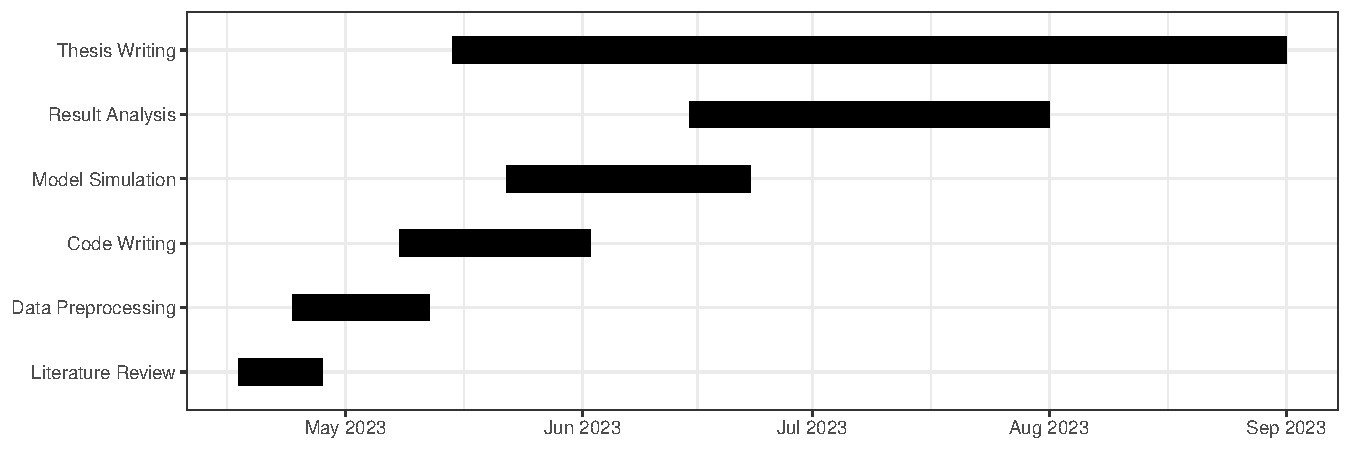
\includegraphics[scale = 0.55]{Gantt_chart.pdf}
    \caption{Gantt chart of the general project plan.}
    \label{fig:Gantt_chart}
\end{figure}

\section{Itemized Budget}

No budget anticipated. 

\bibliographystyle{agsm}
\bibliography{Proposal}

\pagebreak

I have seen and approved the proposal and the budget. \\

Supervisor: Richard Gill\\

Signature: \\

Date: 03/04/2023

\end{spacing}
\end{document}